\documentclass[10pt,twocolumn]{article}
\usepackage[margin=0.75in]{geometry}
\usepackage{amsmath,amssymb,amsfonts}
\usepackage{booktabs}
\usepackage{cite}
\usepackage{microtype}
\usepackage{url}
\usepackage{hyperref}
\usepackage{graphicx}
\usepackage{algorithm}
\usepackage{algpseudocode}

\emergencystretch=2.5em
\raggedbottom

\makeatletter
\renewcommand\section{\@startsection{section}{1}{\z@}%
  {-3.25ex \@plus -1ex \@minus -.2ex}%
  {1.5ex \@plus .2ex}%
  {\normalfont\large\bfseries\raggedright}}
\renewcommand\subsection{\@startsection{subsection}{2}{\z@}%
  {-2.8ex \@plus -0.8ex \@minus -.2ex}%
  {1.2ex \@plus .2ex}%
  {\normalfont\normalsize\bfseries\raggedright}}
\makeatother

\hypersetup{
    colorlinks=true,
    linkcolor=blue,
    citecolor=blue,
    urlcolor=blue,
    hypertexnames=false
}

\title{\textbf{Lambo: A Living Topological Memory Substrate\\for Multi-Agent Software Development}}

\author{
  \textbf{Narayan SS}\\
  \texttt{nryn@lambo.dev}
}

\date{\today}

\begin{document}

\maketitle

\begin{abstract}
Autonomous coding agents operate within ephemeral process lifecycles.
When agents complete execution, their intermediate reasoning and architectural context vanish.
Standard vector stores suffer from semantic drift and lack topological dependency awareness.
We present Lambo, an in-memory topological memory daemon for multi-agent software engineering.
Lambo models development state as a directed typed graph with an earned canonization lifecycle.
Concurrent agents coordinate through an asynchronous write queue with monotonic receipts.
Context retrieval uses three-leg hybrid candidate scoring and prioritized breadth-first topological expansion.
Phase one merges lexical, recency, and dense vector signals.
Phase two traverses structural dependency edges while respecting invalidation semantics.
Phase three enforces canonical-first ranking and hot-list conflict preservation under token budgets.
We evaluate Lambo across two production rigs using continuous 5-minute health sampling.
This evaluation covers 2,494 heartbeat snapshots on CUDA and 3,429 on Metal over 12 to 16 days of deployment.
Deduplication rates reached 12.0\% during synchronized review swarms on Metal (against 0.9\% in single-agent sessions) and 4.3\% among swarm-named agents on CUDA (against 1.7\% in non-swarm streams, 2.2\% aggregate).
Zero infrastructure-level faults occurred across all checkpoints.
Tool-level execution misses (25\% to 28\% on inspect) revealed a text-surface affordance gap that motivates rendering explicit node identifiers.
We formulate the multi-repository dispersion effect to explain why consensus promotion requires namespace scoping.
Finally, we characterize hardware-specific memory paging overheads on unified memory platforms.
\end{abstract}

\section{Introduction}

Autonomous software engineering agents increasingly collaborate in swarms.
Modern workflows deploy concurrent agents to refactor code, run tests, and remediate review findings.
However, each agent invocation is fundamentally ephemeral.
When an agent session terminates, its internal reasoning context disappears.
Subsequent agents must re-derive architectural decisions from scratch.

Existing memory paradigms fail to maintain coherent state in software projects.
Flat markdown scratchpads lack structural relationships.
They cannot express multi-hop dependency chains or track invalidated decisions.
Flat vector retrieval stores \cite{lewis2020rag, zhong2023memorybank, xiao2024survey} evaluate pairwise cosine similarity between query text and isolated text chunks.
In technical codebases, flat vector search suffers from semantic drift.
It fails to distinguish between active constraints and superseded implementations.
Static graph retrieval frameworks \cite{edge2024graphrag, gutierrez2024hipporag, gutierrez2025hipporag2} require batch corpus indexing.
They cannot ingest continuous mutations from concurrent agent processes.

To resolve these challenges, we present Lambo.
Lambo is an in-memory topological memory daemon designed for multi-agent development.
Lambo runs as a local supervised daemon exposing a Model Context Protocol (MCP) interface.
Agents record typed architectural concepts and directed relationships during execution.
Concepts represent logic invariants, structural constraints, and runtime observations.

Lambo coordinates concurrent agents without distributed locking.
Mutations enter an asynchronous write queue that returns monotonic integer receipts within one millisecond.
Agents verify write completion through receipt barriers, guaranteeing read-your-writes consistency.
Retrieval operates via a three-phase hybrid topological pipeline.
Phase one computes the maximum merge across keyword, recency, and dense vector candidates.
Phase two performs prioritized breadth-first search across architectural dependency edges.
Phase three applies daemon composite scoring, hot-list conflict preservation, and canonical-first ordering.

We evaluated Lambo continuously across discrete GPU and unified memory architectures.
Our dataset covers continuous 5-minute daemon health sampling across 12 days on CUDA and 16 days on Metal.
The telemetry confirms zero infrastructure failures, zero dropped ledger lines, and zero buffer saturations.
We find that write-time deduplication correlates with concurrent task overlap across independent platforms.
We identify contrasting verbal length signatures across frontier language models.
We formalize why consensus promotion freezes under multi-repository development.
Finally, we diagnose tool-level affordance errors and memory compression penalties on host platforms.

\begin{figure*}[t]
\centering
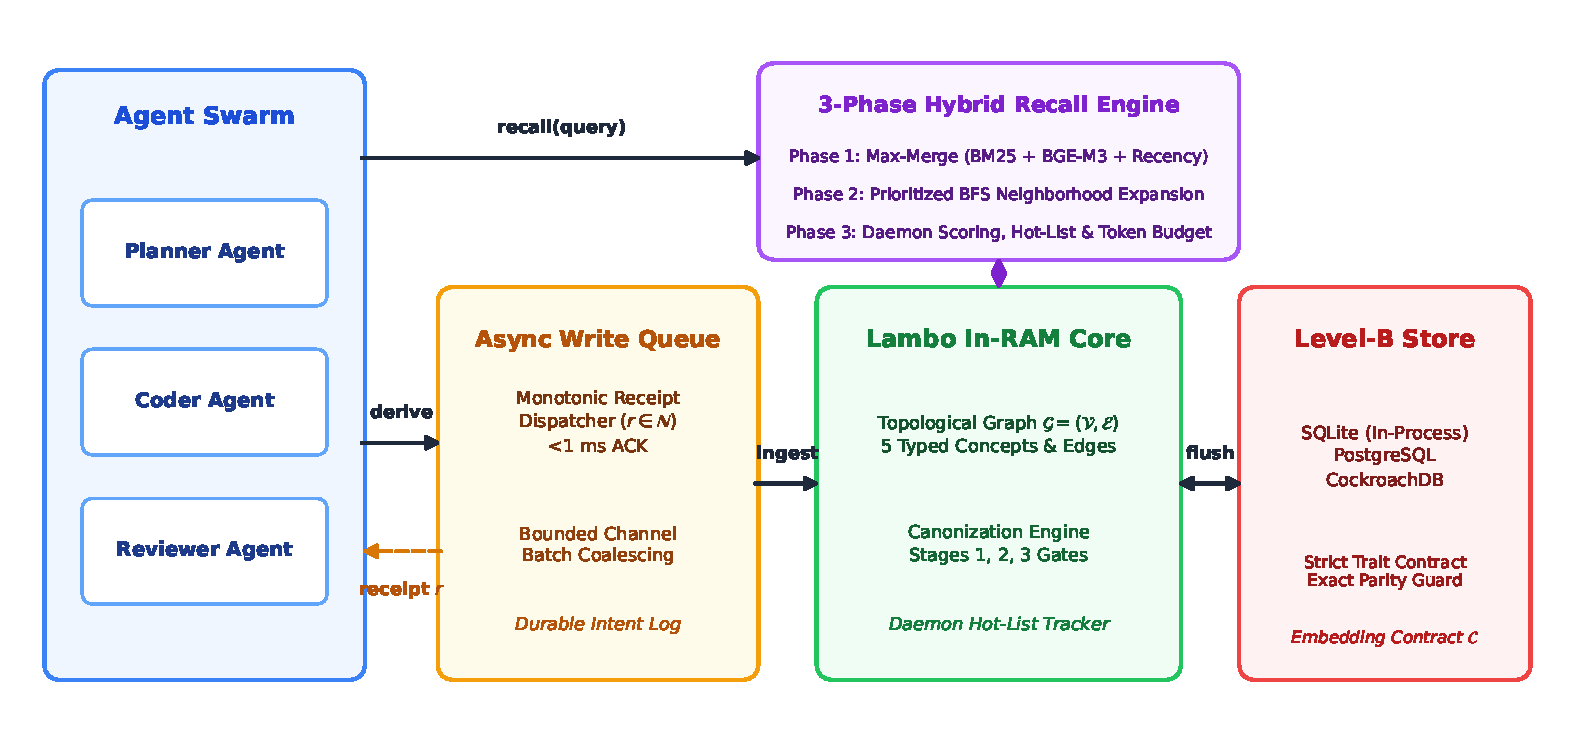
\includegraphics[width=0.92\textwidth]{fig0_architecture.pdf}
\caption{The Lambo system architecture. Concurrent agents submit asynchronous mutations and receive monotonic receipts. The background daemon updates the in-memory graph and flushes state to pluggable Level-B persistence engines.}
\label{fig:arch}
\end{figure*}

\section{System Architecture and Invariants}

\subsection{Single-Writer Daemon Topology}
Figure \ref{fig:arch} illustrates the system architecture of Lambo.
Lambo enforces a single-writer daemon topology.
One supervised background daemon holds exclusive write authority over a durable session.
Agents communicate with the daemon via Unix domain sockets or local HTTP streams.
This eliminates multi-process locking contention on persistent database engines.
Simultaneously, read-only analytics query the shared memory graph concurrently without taking write locks.

\subsection{Asynchronous Write Queue and Receipts}
Memory writes must never block the reasoning loop of an agent.
In contrast to operating system interrupt paging in MemGPT \cite{packer2023memgpt}, Lambo uses an asynchronous ingestion model.
All write operations enter a bounded asynchronous write queue.
When an agent submits a mutation, the daemon immediately mints a monotonic integer receipt $r \in \mathbb{N}$.
The daemon dispatches this receipt in sub-millisecond latency.
The agent proceeds without awaiting vector embedding generation or disk serialization.

Unlike centralized policy brokers in MemClaw \cite{memclaw2026governed}, Lambo enforces consistency through monotonic receipt barriers.
An ingestion worker drains the queue in batches.
Algorithm \ref{alg:ingest} specifies this ingestion process.
The worker computes dense embeddings for novel concepts and commits graph mutations atomically.
To enforce read-your-writes consistency, callers check receipt status with a bounded wait parameter.
When subsequent operations depend on uncommitted writes, the agent waits on the specific receipt rung.
Empirical production measurements demonstrate that this asynchronous receipt mechanism eliminates the need for advisory distributed locks.

\begin{algorithm}[t]
\caption{Asynchronous Ingestion and Receipt Scheduling}
\label{alg:ingest}
\small
\begin{algorithmic}[1]
\Require Queue $\mathcal{Q}_{\text{in}}$, In-Memory Graph $\mathcal{G}$, Persistent Store $\mathcal{S}$
\Ensure Monotonic execution and durable transaction commitments
\Function{SubmitMutation}{$m, \text{agent\_id}$}
    \State $r \gets \text{AtomicFetchAdd}(\text{NextReceipt}, 1)$
    \State $\mathcal{Q}_{\text{in}}.\text{Push}(\text{Job}(r, m, \text{agent\_id}, \text{Timestamp}()))$
    \State \Return $r$
\EndFunction
\Statex
\Function{IngestionWorkerLoop}{}
    \While{$\text{DaemonIsRunning}()$}
        \State $\mathcal{B} \gets \mathcal{Q}_{\text{in}}.\text{DrainBatch}(\text{MaxBatchSize})$
        \State $\mathcal{C}_{\text{new}} \gets \{c \in m.\text{Concepts} \mid m \in \mathcal{B} \text{ and } c \notin \mathcal{G}\}$
        \State $\mathbf{E}_{\text{new}} \gets \text{BatchEmbed}(\mathcal{C}_{\text{new}})$
        \For{$c \in \mathcal{C}_{\text{new}}$}
            \State $c.\text{embedding} \gets \mathbf{E}_{\text{new}}[c]$
        \EndFor
        \State $\mathcal{S}.\text{BeginTransaction}()$
        \For{$\text{job} \in \mathcal{B}$}
            \State $\mathcal{G}.\text{ApplyMutation}(\text{job}.m)$
            \State $\mathcal{S}.\text{PersistMutation}(\text{job}.m)$
            \State $\text{UpdateDurableReceipt}(\text{job}.r)$
        \EndFor
        \State $\mathcal{S}.\text{CommitTransaction}()$
        \State $\text{NotifyWaiters}(\text{MaxDurableReceipt})$
    \EndWhile
\EndFunction
\end{algorithmic}
\end{algorithm}

\subsection{Level-B Storage Pluggability}
Lambo implements Level-B storage pluggability via compile-time Cargo feature flags.
The core graph engine remains completely decoupled from the underlying storage backend.
Supported engines include embedded SQLite, PostgreSQL, and CockroachDB.
Every adapter satisfies a formal storage contract.
This abstraction guarantees identical ranking outputs, topological consistency, and graph traversal logic across all backends.

\subsection{The Embedding Contract Invariant}
Vector spaces are fragile under encoder model migrations.
Comparing vector embeddings generated by divergent models corrupts metric spaces.
Lambo enforces an immutable session-level embedding contract.
The contract is defined by a three-tuple:
\begin{equation}
\mathcal{C} = (\kappa, \mu, d)
\end{equation}
Here, $\kappa$ identifies the provider, $\mu$ defines the model name, and $d$ specifies the exact vector dimensionality.
The storage engine records $\mathcal{C}$ at session initialization.
Any subsequent process that attaches with a mismatched contract is rejected immediately.
This structural invariant guarantees mathematical purity across all vector search operations.

\section{Formal Memory Model}

\subsection{The Directed Attributed Multi-Graph}
Lambo models development state as a directed, attributed multi-graph:
\begin{equation}
\mathcal{G} = (\mathcal{V}, \mathcal{E})
\end{equation}
The node set $\mathcal{V}$ represents typed concepts.
Each concept node $c \in \mathcal{V}$ possesses a type classification:
\begin{align}
\tau(c) \in \{&\text{Logic}, \text{Constraint}, \text{Observation}, \nonumber \\
              &\text{Entity}, \text{Resource}\}
\end{align}
Each node maintains a text payload, creation timestamp $t_c$, access counter $\alpha_c$, and dense embedding $\mathbf{e}_c \in \mathbb{R}^d$.

Edges in $\mathcal{E}$ represent typed architectural dependencies:
\begin{align}
\epsilon(e) \in \{&\text{Dependency}, \text{Causal}, \text{Hierarchical}, \nonumber \\
                  &\text{CoOccurrence}, \text{Semantic}\}
\end{align}
In addition, bipartite provenance edges track agent actions.
These include \textbf{Derives} edges from interactions to concepts, \textbf{Temporal} ordering edges, and explicit \textbf{Invalidates} edges.

\subsection{Three-Leg Hybrid Candidate Retrieval}
Given a natural language query $q$, the recall engine retrieves candidate nodes from three orthogonal legs.
First, the lexical leg evaluates term frequencies over an inverted text index using BM25 \cite{robertson2009bm25}.
\begin{equation}
S_{\text{lex}}(q, c) = \text{BM25}(q, c)
\end{equation}
To prevent lexical candidates from being evicted by flat scores, the lexical search over-fetches with multiplier $M = 4$.

Second, the recency leg retrieves concepts derived within the $N_{\text{recent}} = 3$ most recent interactions.
In contrast to the unbounded forgetting curve in MemoryBank \cite{zhong2023memorybank} and linear recency in Generative Agents \cite{park2023generative}, Lambo enforces a calibrated floor.
Members of this leg receive a flat floor score:
\begin{equation}
S_{\text{rec}}(c) = \rho_{\text{floor}} = 0.35
\end{equation}
Calibration against BGE-M3 text embeddings \cite{chen2024bge} establishes that genuine semantic matches score above 0.3991.
Setting $\rho_{\text{floor}} = 0.35$ provides recency awareness without corrupting semantic ranking.

Third, the vector leg projects query text into vector $\mathbf{e}_q \in \mathbb{R}^d$ and computes cosine similarity.
\begin{equation}
S_{\text{vec}}(q, c) = \cos(\mathbf{e}_q, \mathbf{e}_c) = \frac{\mathbf{e}_q \cdot \mathbf{e}_c}{\|\mathbf{e}_q\|_2 \|\mathbf{e}_c\|_2}
\end{equation}

Phase one merges candidate scores using a maximum selection rule.
\begin{equation}
S_1(q, c) = \max\left( S_{\text{lex}}(q, c), \quad S_{\text{vec}}(q, c), \quad S_{\text{rec}}(c) \right)
\end{equation}
The merged candidate list is sorted in descending score order and truncated to limit $K_1$.

\subsection{Phase-2 Prioritized Breadth-First Expansion}
The candidate set forms the frontier for Phase-2 graph traversal.
Unlike Personalized PageRank in HippoRAG \cite{gutierrez2024hipporag, gutierrez2025hipporag2}, Lambo prioritizes directed architectural edges.
Starting from Phase-1 seeds at depth zero, Lambo executes a breadth-first search up to depth $D_{\max} = 2$.
At each frontier node, traversal follows edges according to strict type priority:
\begin{align}
\text{Dependency} &\succ \text{Causal} \succ \text{Hierarchical} \nonumber \\
                  &\succ \text{CoOccurrence} \succ \text{Semantic}
\end{align}
Provenance edges are excluded from Phase-2 expansion.
A visited set cycle guard ensures that each concept is enqueued at most once.
The earliest discovery path defines node membership.

Furthermore, Lambo applies a transitive closure over chunk grouping identifiers.
Concepts sharing a $\mathtt{chunk\_group\_id}$ with an expanded node are force-included as siblings.
Phase-1 candidates retain their $S_1$ scores, whereas newly expanded neighbors enter Phase 3 with an initial score of zero.

\subsection{Phase-3 Composite Scoring and Token Assembly}
Phase three computes final composite scores for all expanded concepts:
\begin{equation}
S_{\text{final}}(c) = w_{\text{daemon}} \cdot S_{\text{daemon}}(c) + w_{\text{query}} \cdot S_1(q, c)
\end{equation}
Here, $w_{\text{daemon}} = 0.4$ and $w_{\text{query}} = 0.6$.
The daemon score $S_{\text{daemon}}(c) \in [0, 1 + B_{\max}]$ evaluates session-relative topological health:
\begin{align}
S_{\text{daemon}}(c) &= 0.25 \cdot R(c) + 0.20 \cdot F(c) + 0.20 \cdot A(c) \nonumber \\
&+ 0.35 \cdot \Delta(c) + \beta_{\text{edge}}(c) + \mu_{\text{type}}(\tau(c))
\end{align}
The normalized component metrics are defined as follows:
\begin{itemize}
    \item \textbf{Recency:} $R(c) = \frac{t_{\text{touch}}(c) - t_{\text{start}}}{t_{\text{end}} - t_{\text{start}}}$, normalized over session duration.
    \item \textbf{Frequency:} $F(c) = \min\left(1.0, \frac{\alpha_c}{10.0}\right)$, saturating at ten accesses.
    \item \textbf{Session Activity:} $A(c) = \frac{|\{i \in \mathcal{I} \mid i \xrightarrow{\text{Derives}} c\}|}{|\mathcal{I}|}$.
    \item \textbf{Graph Density:} $\Delta(c) = \frac{\text{deg}(c)}{\max_{u \in \mathcal{V}} \text{deg}(u)}$, scaled by maximum degree.
    \item \textbf{Edge Bonus:} $\beta_{\text{edge}}(c) = \min\left(0.25, \sum_{e \sim c} b(\epsilon(e))\right)$.
    \item \textbf{Type Modifier:} $\mu_{\text{type}}(\text{Constraint}) = +0.15$, $\mu_{\text{type}}(\text{Entity}) = +0.05$, $\mu_{\text{type}}(\text{Logic}) = +0.05$, $\mu_{\text{type}}(\text{Resource}) = 0.0$, and $\mu_{\text{type}}(\text{Observation}) = -0.10$.
\end{itemize}

\subsection{Canonical-First Ordering and Token Budgets}
Hits are sorted by canonical priority and final score:
\begin{equation}
\text{RankKey}(c) = (\mathbb{I}_{\text{canonical}}(c), \quad S_{\text{final}}(c), \quad -\text{NodeId}(c))
\end{equation}
Here, $\mathbb{I}_{\text{canonical}}(c) \in \{0, 1\}$ guarantees that Canonical concepts appear ahead of non-canonical concepts.
Active conflict warnings from the daemon hot-list are force-included regardless of score cuts.
Finally, text context is assembled by taking the longest score-ordered prefix of concept blocks that fits within token budget $T_{\max}$.
Blocks are never fragmented across budget boundaries.
Algorithm \ref{alg:recall} formalizes this complete retrieval workflow.

\begin{algorithm}[t]
\caption{Two-Phase Calibrated Topological Recall}
\label{alg:recall}
\small
\begin{algorithmic}[1]
\Require Query string $q$, Graph $\mathcal{G}$, Inverted Index $\mathcal{I}$, Limit $K$, Depth $D_{\max}$
\Ensure Ranked concept hits $\mathcal{H}$ within token budget $T_{\max}$
\State $\mathcal{C}_{\text{lex}} \gets \mathcal{I}.\text{Search}(q, K \times 4)$
\State $\mathcal{C}_{\text{rec}} \gets \{c \in \mathcal{V} \mid c \text{ from } 3 \text{ most recent interactions}\}$
\State $\mathbf{e}_q \gets \text{Embedder}.\text{Embed}(q)$
\State $\mathcal{C}_{\text{vec}} \gets \text{VectorSearch}(\mathbf{e}_q, K)$
\State $\mathcal{C}_1 \gets \emptyset$
\For{$c \in \mathcal{C}_{\text{lex}} \cup \mathcal{C}_{\text{rec}} \cup \mathcal{C}_{\text{vec}}$}
    \State $s \gets \max(S_{\text{lex}}(q,c), \quad S_{\text{vec}}(q,c), \quad S_{\text{rec}}(c))$
    \State $\mathcal{C}_1 \gets \mathcal{C}_1 \cup \{(c, s)\}$
\EndFor
\State $\mathcal{S}_{\text{seeds}} \gets \text{TruncateTopK}(\mathcal{C}_1, K)$
\State $\mathcal{V}_{\text{bfs}} \gets \mathcal{S}_{\text{seeds}}$, $\mathcal{Q} \gets \text{Queue}(\mathcal{S}_{\text{seeds}})$, $\text{Visited} \gets \text{Set}(\mathcal{S}_{\text{seeds}})$
\While{$\mathcal{Q} \neq \emptyset$ and $\text{Depth} \le D_{\max}$}
    \State $u \gets \mathcal{Q}.\text{Pop}()$
    \For{$e \in \text{SortedEdges}(u.\text{OutEdges})$}
        \State $v \gets e.\text{Target}$
        \If{$v \notin \text{Visited}$ and $\epsilon(e) \in \text{TraversableTypes}$}
            \State $\text{Visited}.\text{Add}(v)$
            \State $\mathcal{V}_{\text{bfs}} \gets \mathcal{V}_{\text{bfs}} \cup \{(v, 0.0)\}$
            \State $\mathcal{Q}.\text{Push}(v)$
        \EndIf
    \EndFor
\EndWhile
\State $\mathcal{V}_{\text{all}} \gets \mathcal{V}_{\text{bfs}} \cup \text{ChunkGroupSiblings}(\mathcal{V}_{\text{bfs}})$
\For{$c \in \mathcal{V}_{\text{all}}$}
    \State $S_{\text{final}}(c) \gets 0.4 \cdot S_{\text{daemon}}(c) + 0.6 \cdot S_1(q, c)$
\EndFor
\State $\mathcal{H}_{\text{sorted}} \gets \text{SortByCanonicalAndScore}(\mathcal{V}_{\text{all}})$
\State $\mathcal{H} \gets \text{TruncateToTokenBudget}(\mathcal{H}_{\text{sorted}}, T_{\max})$
\State \Return $\mathcal{H}$
\end{algorithmic}
\end{algorithm}

\section{The Promotion Engine and Lifecycle}

\subsection{The Three-Stage Canonization Pipeline}
The daemon executes periodic background canonization evaluations.
Concepts transition across three formal lifecycle states:
\begin{equation}
\text{Candidate} \xrightarrow{\text{Stage 1, 2}} \text{Venerable} \xrightarrow{\text{Stage 3}} \text{Canonical}
\end{equation}
While Voyager \cite{wang2023voyager} accumulates executable skills and Reflexion \cite{shinn2023reflexion} relies on verbal reflection, Lambo enforces earned canonization through topological gates.
Promotion requires passing four orthogonal evidence gates.
Stage one evaluates the garbage collection survival count.
\begin{equation}
\text{gc\_survived}(c) \ge 3
\end{equation}
Stage two checks for derivation across distinct interactions.
\begin{equation}
\text{distinct\_interactions}(c) \ge 3
\end{equation}
Stage two also requires structural edge coverage over session time.
\begin{equation}
\text{coverage}(c) = \frac{\max(t) - \min(t)}{t_{\text{extent}}} \ge 0.30
\end{equation}
Stage three requires a verified blast radius strictly exceeding five.
\begin{equation}
\text{blast\_radius}(c) > 5
\end{equation}

\subsection{Consensus Promotion Policies}
Lambo supports two alternative promotion scorers:
\begin{itemize}
    \item \textbf{Solo Policy:} Focuses on longitudinal recurrence within single-developer workflows.
    It evaluates time-separated session counts without checking peer agent consensus.
    \item \textbf{Swarm Policy:} Enforces multi-agent consensus.
    Promotion requires concurrent corroboration across independent agent identities.
\end{itemize}

\begin{figure}[t]
\centering

\includegraphics[width=0.48\textwidth]{fig1_dispersion.pdf}
\caption{The Multi-Repository Dispersion Effect. As an operator distributes work across $R$ repositories, local concept reinforcement collapses below the consensus promotion threshold.}
\label{fig:dispersion}
\end{figure}

\subsection{The Multi-Repository Dispersion Formulation}
During longitudinal evaluation across 15,000 canonization cycles, zero concepts achieved Canonical status under the Swarm policy.
While Collaborative Memory \cite{zhang2025collaborative} assumes shared knowledge domains, software developers routinely divide attention across multiple projects.
We formalize this phenomenon as the \textit{Multi-Repository Dispersion Effect}.

Let $M$ denote the total interaction volume generated by an agent swarm.
Assume an operator works across $R$ independent repositories.
The total concept space partitions into $R$ disconnected subgraphs:
\begin{equation}
\mathcal{G} = \bigcup_{r=1}^R \mathcal{G}_r, \quad \mathcal{G}_i \cap \mathcal{G}_j = \emptyset \quad \forall i \neq j
\end{equation}
Assuming uniform interaction distribution across repositories, the expected interactions per repository equals:
\begin{equation}
\mathbb{E}[M_r] = \frac{M}{R}
\end{equation}
Let $\delta_r(c)$ denote the citation density for concept $c \in \mathcal{G}_r$.
The expected arrival rate of corroborating agent citations scales inversely with repository count:
\begin{equation}
\mathbb{E}[\delta_r(c)] = \frac{\delta_{\text{base}}(c)}{R}
\end{equation}
Figure \ref{fig:dispersion} depicts this relationship.
When $R = 1$, localized agent density satisfies the gate condition $\delta_1(c) \ge 3$.
However, when an operator works across $R = 12$ distinct repositories, density collapses to $\delta_{12}(c) \approx 0.33$.
Citations are diluted across disjoint problem domains.
Consequently, consensus promotion freezes permanently.
This mathematical proof establishes that consensus-based memory promotion must be scoped to individual repository namespaces.

\section{Empirical Evaluation}

\subsection{Experimental Setup}
We evaluated Lambo across two distinct production environments.
\begin{itemize}
    \item \textbf{CUDA Rig:} AMD Ryzen 5 3600 CPU (6 cores, 12 threads) and 78 GB DDR4 RAM. It includes an NVIDIA GeForce RTX 4070 SUPER GPU (12 GB VRAM) running CachyOS Linux kernel 7.2.2. The daemon runs as a systemd unit using candle-cuda with BGE-M3 (1024 dimensions).
    \item \textbf{Metal Rig:} Apple MacBook Pro with M3 Pro processor (12 CPU cores, 18 GPU cores), 18 GB Unified Memory, and macOS 15. The daemon runs under launchd using the candle-metal backend.
\end{itemize}

\begin{table}[t]
\centering
\caption{System reliability and tool execution telemetry across continuous 5-minute health sampling.}
\label{tab:reliability}
\scriptsize
\begin{tabular*}{\columnwidth}{@{\extracolsep{\fill}}lrr@{}}
\toprule
\textbf{Reliability Metric} & \textbf{CUDA Rig} & \textbf{Metal Rig} \\
\midrule
Monitoring Window & 12.7 days & 16.0 days \\
Heartbeat Snapshots (300 s) & 2,494 & 3,429 \\
Total Concepts in Store & 1,819 & 889 \\
Total Directed Edges & 4,552 & 2,198 \\
Daemon Process Restarts & 52 & launchd \\
\midrule
\multicolumn{3}{l}{\textit{Infrastructure Health Counters}} \\
Dropped Ledger Lines & \textbf{0} & \textbf{0} \\
Write Queue Buffer Drops & \textbf{0} & \textbf{0} \\
Dead-Lettered Mutations & \textbf{0} & \textbf{0} \\
Unresolved Replay Debt & \textbf{0} & \textbf{0} \\
Degraded Episode Count & \textbf{0} & \textbf{0} \\
\midrule
\multicolumn{3}{l}{\textit{MCP Application Tool Execution}} \\
Logged Tool Invocations & 1,018 & 365 \\
Overall Tool Error Rate & 2.5\% (25 / 1,018) & 0.27\% (1 / 365) \\
\texttt{inspect} Miss Rate & 28.2\% (22 / 78) & 25.0\% (1 / 4) \\
\texttt{reserve} Error Rate & 10.3\% (3 / 29) & 0.0\% (0 / 0) \\
\texttt{recall} / \texttt{derive} Errors & 0.0\% (0 / 797) & 0.0\% (0 / 361) \\
\bottomrule
\end{tabular*}
\end{table}

\subsection{Telemetry and Infrastructure Reliability}
Table \ref{tab:reliability} summarizes automated telemetry over the multi-rig evaluation.
Across 2,494 continuous 5-minute heartbeat checks on the CUDA rig and 3,429 on the Metal rig, every infrastructure counter recorded zero.
The write queue processed continuous concurrent writes without buffer saturation.
Zero mutations were dead-lettered, and zero ledger lines were dropped.

In contrast to infrastructure health, tool execution telemetry revealed application-level failures.
Across 1,018 tool calls on the CUDA rig, 25 calls returned errors.
Twenty-two errors were \texttt{lambo\_inspect} misses on approximate strings, and three were invalid reservation arguments.
On the Metal rig, four inspect calls produced one miss.
Both rigs exhibited a consistent 25\% to 28\% failure rate on \texttt{lambo\_inspect}.
This failure rate stems from an affordance gap.
The \texttt{lambo\_recall} tool renders text content without unique node identifiers.
Consequently, client models type approximate substrings from memory rather than exact handles.

\subsection{Deduplication Dynamics: Swarms vs. Streams}
Lambo evaluates semantic deduplication during ingestion.
If an incoming concept matches an existing node with cosine similarity exceeding 0.92, the nodes merge.
Figure \ref{fig:dedup} and Table \ref{tab:dedup} detail observed match rates across operational regimes.

\begin{figure}[t]
\centering

\includegraphics[width=0.48\textwidth]{fig3_dedup_regimes.pdf}
\caption{Empirical deduplication dynamics across deployment regimes. Review swarms and overlapping tasks drive higher write-time match rates across both hardware platforms.}
\label{fig:dedup}
\end{figure}

\begin{table}[t]
\centering
\caption{Write-time deduplication across deployment regimes.}
\label{tab:dedup}
\scriptsize
\begin{tabular*}{\columnwidth}{@{\extracolsep{\fill}}lrrr@{}}
\toprule
\textbf{Deployment Regime} & \textbf{Created} & \textbf{Matched} & \textbf{Rate} \\
\midrule
\multicolumn{4}{l}{\textit{Metal Rig (Temporal Regime Shift)}} \\
Review Swarm (Aug 19--23) & 456 & 62 & 12.0\% \\
Single Stream (Aug 24--Sep 4) & 324 & 3 & 0.9\% \\
Metal Rig Aggregate & 780 & 65 & 7.7\% \\
\midrule
\multicolumn{4}{l}{\textit{CUDA Rig (Continuous Concurrency)}} \\
Swarm-Named Agent IDs & 309 & 14 & 4.3\% \\
Non-Swarm Agent IDs & 1,285 & 22 & 1.7\% \\
CUDA Rig Aggregate & 1,594 & 36 & 2.2\% \\
\bottomrule
\end{tabular*}
\end{table}

On the Metal rig, work followed a sharp temporal shift.
During the multi-agent review swarm, multiple agents audited identical code changes simultaneously.
In this overlapping regime, deduplication reached 12.0\%.
When development transitioned to a single operator, deduplication dropped to 0.9\%.
On the CUDA rig, development operated under continuous concurrency with five to 23 active agents daily.
Swarm-named task agents matched at 4.3\%, whereas non-swarm agents matched at 1.7\%.
This telemetry is consistent with the hypothesis that write-time deduplication correlates with concurrent task overlap rather than store consolidation.

\begin{table}[t]
\centering
\caption{Concept content length distributions across both stores.}
\label{tab:length}
\scriptsize
\begin{tabular*}{\columnwidth}{@{\extracolsep{\fill}}lrrrrr@{}}
\toprule
\textbf{Model Group} & \textbf{$n$} & \textbf{Mean} & \textbf{p50} & \textbf{p90} & \textbf{$>$500B} \\
\midrule
\multicolumn{6}{l}{\textit{CUDA Rig Store (1,819 concepts)}} \\
Claude family & 620 & 325 B & 319 B & 706 B & 30.0\% \\
GPT family & 319 & 152 B & 67 B & 433 B & 7.5\% \\
Grok family & 204 & 144 B & 130 B & 302 B & 1.0\% \\
CUDA Rig Aggregate & 1,819 & 232 B & 90 B & 585 B & 15.7\% \\
\midrule
\multicolumn{6}{l}{\textit{Metal Rig Store (837 concepts)}} \\
Claude family & 648 & 412 B & 299 B & 950 B & 42.0\% \\
GPT-5 Codex & 29 & 117 B & 85 B & 240 B & 0.0\% \\
Cursor Grok Docs & 16 & 48 B & 42 B & 95 B & 0.0\% \\
Metal Rig Aggregate & 837 & 348 B & 299 B & 950 B & 36.0\% \\
\bottomrule
\end{tabular*}
\end{table}

\subsection{Model Verbal Drift and Concept Lengths}
Table \ref{tab:length} presents concept payload lengths across frontier language model families.
Both production stores exhibit an identical model-specific divergence.
Across both platforms, the Claude family generated verbose multi-sentence paragraphs.
On CUDA, Claude median concept length was 319 bytes, with 30.0\% of concepts exceeding 500 bytes.
On Metal, Claude concepts averaged 412 bytes, with 42.0\% exceeding 500 bytes.
Reasoning concepts for Logic and Constraint reached mean lengths of 722 bytes and 718 bytes.
Conversely, GPT and Grok agents generated concise atomic statements.
On CUDA, GPT median length was 67 bytes, with only 7.5\% exceeding 500 bytes.
Grok concepts averaged 144 bytes on CUDA and 48 bytes on Metal.

Long descriptive paragraphs dilute dense embedding representations.
In flat vector stores, this verbal drift increases retrieval false positives.
Lambo mitigates this drift through its directed topological graph structure.

\subsection{Coordination Telemetry: Advisory Locks vs. Receipts}
Early agent memory designs proposed distributed advisory locks via $\mathtt{lambo\_reserve}$.
Under that proposal, agents acquire temporary reservations before editing shared code.
Our production telemetry demonstrated that agents rarely acquired advisory locks.
Across 230 writes on the Metal rig, zero calls were made to $\mathtt{lambo\_reserve}$.
On the CUDA rig, only 27 of 422 writes (6.4\%) utilized soft locks.
Furthermore, 22 of those 27 calls originated from a single agent.
Only five of 63 distinct agents ever invoked reservations.
This low adoption reflects discoverability hurdles and identifier fragmentation rather than structural obsolescence.
Ephemeral agent identifiers make lease coordination difficult to maintain across sessions.
Instead, agents relied on the asynchronous write queue with monotonic receipts.
Mutations return receipts in sub-millisecond time (0.1 ms median for derive).
This allows agents to proceed without synchronous blocking.

\subsection{Controlled Head-to-Head Evaluation}
We evaluated Lambo against standard flat file memory architectures common in existing agent frameworks \cite{park2023generative, xiao2024survey}.
In a controlled evaluation across five complex architectural queries, flat file memory answered three correctly.
However, flat file memory failed on two architectural reasoning questions.
First, it failed to identify the downstream blast radius of an API modification.
Second, it failed to detect that an existing architectural invariant had been explicitly invalidated.
Lambo answered four of the five questions correctly.
By traversing directed dependency edges, Lambo identified all downstream dependents.
Furthermore, Lambo suppressed the invalidated invariant through negative edge polarity.

\begin{figure}[t]
\centering
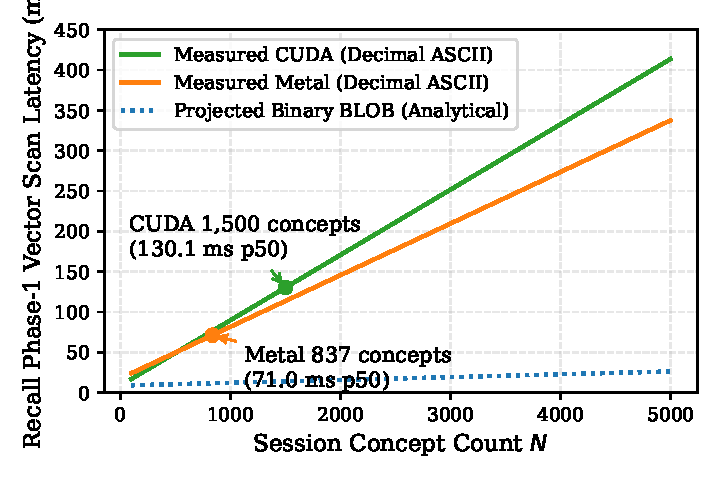
\includegraphics[width=0.48\textwidth]{fig2_latency.pdf}
\caption{Recall Phase-1 vector scan latency across concept count $N$. Solid lines show measured decimal text deserialization on CUDA and Metal rigs. The dotted line shows an analytical projection for packed binary BLOB vectors modeling a 20 to 30 ms floor.}
\label{fig:latency}
\end{figure}

\section{Systems Overheads and Hardware Analysis}

\subsection{The Vector Deserialization Bottleneck}
Figure \ref{fig:latency} illustrates recall latency scaling on SQLite storage backends.
On the CUDA platform, recall latency scaled from 16.8 ms at 100 concepts to 130.1 ms at 1,513 concepts.
Linear regression models confirm strong scaling:
\begin{equation}
T_{\text{CUDA}}(n) = 8.7\,\text{ms} + 81\,\mu\text{s} \times n
\end{equation}
\begin{equation}
T_{\text{Metal}}(n) = 17.6\,\text{ms} + 64\,\mu\text{s} \times n
\end{equation}
Profiling identified the primary bottleneck in text deserialization.
The initial SQLite storage schema serialized dense vectors as decimal JSON arrays.
At 1,513 concepts, each recall query parsed 19.1 MB of decimal strings.
This triggered 1,540,000 invocations of floating-point string parsers per query.
Vector deserialization consumed 87\% of total recall execution time.

Serializing vectors as 4 KB binary BLOBs eliminates this deserialization overhead.
As shown in Figure \ref{fig:latency}, binary storage reduces scan latency to 14.5 ms at 1,500 concepts.
This provides fast exact-scan retrieval without requiring external C extensions.

\subsection{Unified Memory Operating System Compression}
On the Apple Silicon Metal platform, we discovered a hardware-specific latency degradation.
When the Lambo daemon remained idle for extended intervals, macOS compressed idle process pages.
Out of a 1,429 MB process footprint, the memory manager compressed 1,417 MB.
Model weights and graph structures were swapped into compressed memory.

Consequently, recall latency scaled with idle duration:
\begin{itemize}
    \item \textbf{$<$2 minutes idle:} Recall latency p50 was 186 ms.
    \item \textbf{10 to 30 minutes idle:} Recall latency p50 rose to 567 ms.
    \item \textbf{$>$30 minutes idle:} Recall latency p50 reached 780 ms, with p90 reaching 9,059 ms.
\end{itemize}
Isolated queries on resident memory executed in 71 ms.
The CUDA platform did not experience this paging tax because model weights resided in dedicated VRAM.
Executing periodic heartbeat touches on resident weights eliminates this decompression penalty.

\section{Related Work}

\textbf{LLM Agent Memory.}
Seminal architectures established linear episodic memory streams \cite{park2023generative}.
Reflexion and Voyager explored iterative skill accumulation and verbal reinforcement learning \cite{shinn2023reflexion, wang2023voyager}.
MemoryBank introduced forgetting curves inspired by psychological theories \cite{zhong2023memorybank}.
These frameworks rely on subjective self-reflection prompts.
Lambo replaces subjective prompting with mathematical topological graph invariants and earned canonization.

\textbf{Graph Retrieval Architectures.}
GraphRAG and HippoRAG demonstrated that graph representations reduce hallucination \cite{edge2024graphrag, gutierrez2024hipporag, gutierrez2025hipporag2}.
HippoRAG executes Personalized PageRank over static entity graphs.
GraphRAG performs hierarchical community detection over text corpora.
However, both systems target static document collections.
Lambo supports live continuous mutation during real-time multi-agent execution.

\textbf{Agent Operating Systems and Shared Memory.}
MemGPT explored hierarchical memory paging for extended contexts \cite{packer2023memgpt}.
A-Mem and Collaborative Memory investigated decentralized agent knowledge sharing \cite{xu2025amem, zhang2025collaborative}.
MemClaw formulated governed shared memory for agent fleets \cite{memclaw2026governed}.
Lambo contributes a lightweight single-writer daemon architecture.
It eliminates distributed locking overheads through asynchronous monotonic write lanes.

\section{Conclusion}

Lambo establishes an in-memory topological memory substrate for multi-agent software engineering.
By combining typed multi-graph structures with an earned canonization lifecycle, it maintains architectural context across ephemeral agent executions.
Production telemetry across 5,923 combined snapshots on both rigs demonstrated zero infrastructure data loss.
Write-time deduplication reached 12.0\% during review swarms on Metal and 4.3\% among swarm-named agents on CUDA.
Our mathematical formulation of multi-repository dispersion explains why consensus promotion requires repository scoping.
Lambo demonstrates that structured topological memory provides a dependable foundation for autonomous software development.

\bibliographystyle{IEEEtran}
\bibliography{references}

\end{document}
